
% Default to the notebook output style

    


% Inherit from the specified cell style.




    
\documentclass[11pt]{article}

    
    
    \usepackage[T1]{fontenc}
    % Nicer default font (+ math font) than Computer Modern for most use cases
    \usepackage{mathpazo}

    % Basic figure setup, for now with no caption control since it's done
    % automatically by Pandoc (which extracts ![](path) syntax from Markdown).
    \usepackage{graphicx}
    % We will generate all images so they have a width \maxwidth. This means
    % that they will get their normal width if they fit onto the page, but
    % are scaled down if they would overflow the margins.
    \makeatletter
    \def\maxwidth{\ifdim\Gin@nat@width>\linewidth\linewidth
    \else\Gin@nat@width\fi}
    \makeatother
    \let\Oldincludegraphics\includegraphics
    % Set max figure width to be 80% of text width, for now hardcoded.
    \renewcommand{\includegraphics}[1]{\Oldincludegraphics[width=.8\maxwidth]{#1}}
    % Ensure that by default, figures have no caption (until we provide a
    % proper Figure object with a Caption API and a way to capture that
    % in the conversion process - todo).
    \usepackage{caption}
    \DeclareCaptionLabelFormat{nolabel}{}
    \captionsetup{labelformat=nolabel}

    \usepackage{adjustbox} % Used to constrain images to a maximum size 
    \usepackage{xcolor} % Allow colors to be defined
    \usepackage{enumerate} % Needed for markdown enumerations to work
    \usepackage{geometry} % Used to adjust the document margins
    \usepackage{amsmath} % Equations
    \usepackage{amssymb} % Equations
    \usepackage{textcomp} % defines textquotesingle
    % Hack from http://tex.stackexchange.com/a/47451/13684:
    \AtBeginDocument{%
        \def\PYZsq{\textquotesingle}% Upright quotes in Pygmentized code
    }
    \usepackage{upquote} % Upright quotes for verbatim code
    \usepackage{eurosym} % defines \euro
    \usepackage[mathletters]{ucs} % Extended unicode (utf-8) support
    \usepackage[utf8x]{inputenc} % Allow utf-8 characters in the tex document
    \usepackage{fancyvrb} % verbatim replacement that allows latex
    \usepackage{grffile} % extends the file name processing of package graphics 
                         % to support a larger range 
    % The hyperref package gives us a pdf with properly built
    % internal navigation ('pdf bookmarks' for the table of contents,
    % internal cross-reference links, web links for URLs, etc.)
    \usepackage{hyperref}
    \usepackage{longtable} % longtable support required by pandoc >1.10
    \usepackage{booktabs}  % table support for pandoc > 1.12.2
    \usepackage[inline]{enumitem} % IRkernel/repr support (it uses the enumerate* environment)
    \usepackage[normalem]{ulem} % ulem is needed to support strikethroughs (\sout)
                                % normalem makes italics be italics, not underlines
    

    
    
    % Colors for the hyperref package
    \definecolor{urlcolor}{rgb}{0,.145,.698}
    \definecolor{linkcolor}{rgb}{.71,0.21,0.01}
    \definecolor{citecolor}{rgb}{.12,.54,.11}

    % ANSI colors
    \definecolor{ansi-black}{HTML}{3E424D}
    \definecolor{ansi-black-intense}{HTML}{282C36}
    \definecolor{ansi-red}{HTML}{E75C58}
    \definecolor{ansi-red-intense}{HTML}{B22B31}
    \definecolor{ansi-green}{HTML}{00A250}
    \definecolor{ansi-green-intense}{HTML}{007427}
    \definecolor{ansi-yellow}{HTML}{DDB62B}
    \definecolor{ansi-yellow-intense}{HTML}{B27D12}
    \definecolor{ansi-blue}{HTML}{208FFB}
    \definecolor{ansi-blue-intense}{HTML}{0065CA}
    \definecolor{ansi-magenta}{HTML}{D160C4}
    \definecolor{ansi-magenta-intense}{HTML}{A03196}
    \definecolor{ansi-cyan}{HTML}{60C6C8}
    \definecolor{ansi-cyan-intense}{HTML}{258F8F}
    \definecolor{ansi-white}{HTML}{C5C1B4}
    \definecolor{ansi-white-intense}{HTML}{A1A6B2}

    % commands and environments needed by pandoc snippets
    % extracted from the output of `pandoc -s`
    \providecommand{\tightlist}{%
      \setlength{\itemsep}{0pt}\setlength{\parskip}{0pt}}
    \DefineVerbatimEnvironment{Highlighting}{Verbatim}{commandchars=\\\{\}}
    % Add ',fontsize=\small' for more characters per line
    \newenvironment{Shaded}{}{}
    \newcommand{\KeywordTok}[1]{\textcolor[rgb]{0.00,0.44,0.13}{\textbf{{#1}}}}
    \newcommand{\DataTypeTok}[1]{\textcolor[rgb]{0.56,0.13,0.00}{{#1}}}
    \newcommand{\DecValTok}[1]{\textcolor[rgb]{0.25,0.63,0.44}{{#1}}}
    \newcommand{\BaseNTok}[1]{\textcolor[rgb]{0.25,0.63,0.44}{{#1}}}
    \newcommand{\FloatTok}[1]{\textcolor[rgb]{0.25,0.63,0.44}{{#1}}}
    \newcommand{\CharTok}[1]{\textcolor[rgb]{0.25,0.44,0.63}{{#1}}}
    \newcommand{\StringTok}[1]{\textcolor[rgb]{0.25,0.44,0.63}{{#1}}}
    \newcommand{\CommentTok}[1]{\textcolor[rgb]{0.38,0.63,0.69}{\textit{{#1}}}}
    \newcommand{\OtherTok}[1]{\textcolor[rgb]{0.00,0.44,0.13}{{#1}}}
    \newcommand{\AlertTok}[1]{\textcolor[rgb]{1.00,0.00,0.00}{\textbf{{#1}}}}
    \newcommand{\FunctionTok}[1]{\textcolor[rgb]{0.02,0.16,0.49}{{#1}}}
    \newcommand{\RegionMarkerTok}[1]{{#1}}
    \newcommand{\ErrorTok}[1]{\textcolor[rgb]{1.00,0.00,0.00}{\textbf{{#1}}}}
    \newcommand{\NormalTok}[1]{{#1}}
    
    % Additional commands for more recent versions of Pandoc
    \newcommand{\ConstantTok}[1]{\textcolor[rgb]{0.53,0.00,0.00}{{#1}}}
    \newcommand{\SpecialCharTok}[1]{\textcolor[rgb]{0.25,0.44,0.63}{{#1}}}
    \newcommand{\VerbatimStringTok}[1]{\textcolor[rgb]{0.25,0.44,0.63}{{#1}}}
    \newcommand{\SpecialStringTok}[1]{\textcolor[rgb]{0.73,0.40,0.53}{{#1}}}
    \newcommand{\ImportTok}[1]{{#1}}
    \newcommand{\DocumentationTok}[1]{\textcolor[rgb]{0.73,0.13,0.13}{\textit{{#1}}}}
    \newcommand{\AnnotationTok}[1]{\textcolor[rgb]{0.38,0.63,0.69}{\textbf{\textit{{#1}}}}}
    \newcommand{\CommentVarTok}[1]{\textcolor[rgb]{0.38,0.63,0.69}{\textbf{\textit{{#1}}}}}
    \newcommand{\VariableTok}[1]{\textcolor[rgb]{0.10,0.09,0.49}{{#1}}}
    \newcommand{\ControlFlowTok}[1]{\textcolor[rgb]{0.00,0.44,0.13}{\textbf{{#1}}}}
    \newcommand{\OperatorTok}[1]{\textcolor[rgb]{0.40,0.40,0.40}{{#1}}}
    \newcommand{\BuiltInTok}[1]{{#1}}
    \newcommand{\ExtensionTok}[1]{{#1}}
    \newcommand{\PreprocessorTok}[1]{\textcolor[rgb]{0.74,0.48,0.00}{{#1}}}
    \newcommand{\AttributeTok}[1]{\textcolor[rgb]{0.49,0.56,0.16}{{#1}}}
    \newcommand{\InformationTok}[1]{\textcolor[rgb]{0.38,0.63,0.69}{\textbf{\textit{{#1}}}}}
    \newcommand{\WarningTok}[1]{\textcolor[rgb]{0.38,0.63,0.69}{\textbf{\textit{{#1}}}}}
    
    
    % Define a nice break command that doesn't care if a line doesn't already
    % exist.
    \def\br{\hspace*{\fill} \\* }
    % Math Jax compatability definitions
    \def\gt{>}
    \def\lt{<}
    % Document parameters
    \title{Chapter4\_answer}
    
    
    

    % Pygments definitions
    
\makeatletter
\def\PY@reset{\let\PY@it=\relax \let\PY@bf=\relax%
    \let\PY@ul=\relax \let\PY@tc=\relax%
    \let\PY@bc=\relax \let\PY@ff=\relax}
\def\PY@tok#1{\csname PY@tok@#1\endcsname}
\def\PY@toks#1+{\ifx\relax#1\empty\else%
    \PY@tok{#1}\expandafter\PY@toks\fi}
\def\PY@do#1{\PY@bc{\PY@tc{\PY@ul{%
    \PY@it{\PY@bf{\PY@ff{#1}}}}}}}
\def\PY#1#2{\PY@reset\PY@toks#1+\relax+\PY@do{#2}}

\expandafter\def\csname PY@tok@sc\endcsname{\def\PY@tc##1{\textcolor[rgb]{0.73,0.13,0.13}{##1}}}
\expandafter\def\csname PY@tok@mf\endcsname{\def\PY@tc##1{\textcolor[rgb]{0.40,0.40,0.40}{##1}}}
\expandafter\def\csname PY@tok@gt\endcsname{\def\PY@tc##1{\textcolor[rgb]{0.00,0.27,0.87}{##1}}}
\expandafter\def\csname PY@tok@ge\endcsname{\let\PY@it=\textit}
\expandafter\def\csname PY@tok@nc\endcsname{\let\PY@bf=\textbf\def\PY@tc##1{\textcolor[rgb]{0.00,0.00,1.00}{##1}}}
\expandafter\def\csname PY@tok@kr\endcsname{\let\PY@bf=\textbf\def\PY@tc##1{\textcolor[rgb]{0.00,0.50,0.00}{##1}}}
\expandafter\def\csname PY@tok@sh\endcsname{\def\PY@tc##1{\textcolor[rgb]{0.73,0.13,0.13}{##1}}}
\expandafter\def\csname PY@tok@c1\endcsname{\let\PY@it=\textit\def\PY@tc##1{\textcolor[rgb]{0.25,0.50,0.50}{##1}}}
\expandafter\def\csname PY@tok@ow\endcsname{\let\PY@bf=\textbf\def\PY@tc##1{\textcolor[rgb]{0.67,0.13,1.00}{##1}}}
\expandafter\def\csname PY@tok@gd\endcsname{\def\PY@tc##1{\textcolor[rgb]{0.63,0.00,0.00}{##1}}}
\expandafter\def\csname PY@tok@il\endcsname{\def\PY@tc##1{\textcolor[rgb]{0.40,0.40,0.40}{##1}}}
\expandafter\def\csname PY@tok@sb\endcsname{\def\PY@tc##1{\textcolor[rgb]{0.73,0.13,0.13}{##1}}}
\expandafter\def\csname PY@tok@s1\endcsname{\def\PY@tc##1{\textcolor[rgb]{0.73,0.13,0.13}{##1}}}
\expandafter\def\csname PY@tok@cpf\endcsname{\let\PY@it=\textit\def\PY@tc##1{\textcolor[rgb]{0.25,0.50,0.50}{##1}}}
\expandafter\def\csname PY@tok@gp\endcsname{\let\PY@bf=\textbf\def\PY@tc##1{\textcolor[rgb]{0.00,0.00,0.50}{##1}}}
\expandafter\def\csname PY@tok@k\endcsname{\let\PY@bf=\textbf\def\PY@tc##1{\textcolor[rgb]{0.00,0.50,0.00}{##1}}}
\expandafter\def\csname PY@tok@gr\endcsname{\def\PY@tc##1{\textcolor[rgb]{1.00,0.00,0.00}{##1}}}
\expandafter\def\csname PY@tok@dl\endcsname{\def\PY@tc##1{\textcolor[rgb]{0.73,0.13,0.13}{##1}}}
\expandafter\def\csname PY@tok@gh\endcsname{\let\PY@bf=\textbf\def\PY@tc##1{\textcolor[rgb]{0.00,0.00,0.50}{##1}}}
\expandafter\def\csname PY@tok@se\endcsname{\let\PY@bf=\textbf\def\PY@tc##1{\textcolor[rgb]{0.73,0.40,0.13}{##1}}}
\expandafter\def\csname PY@tok@mh\endcsname{\def\PY@tc##1{\textcolor[rgb]{0.40,0.40,0.40}{##1}}}
\expandafter\def\csname PY@tok@nl\endcsname{\def\PY@tc##1{\textcolor[rgb]{0.63,0.63,0.00}{##1}}}
\expandafter\def\csname PY@tok@ch\endcsname{\let\PY@it=\textit\def\PY@tc##1{\textcolor[rgb]{0.25,0.50,0.50}{##1}}}
\expandafter\def\csname PY@tok@ni\endcsname{\let\PY@bf=\textbf\def\PY@tc##1{\textcolor[rgb]{0.60,0.60,0.60}{##1}}}
\expandafter\def\csname PY@tok@kt\endcsname{\def\PY@tc##1{\textcolor[rgb]{0.69,0.00,0.25}{##1}}}
\expandafter\def\csname PY@tok@m\endcsname{\def\PY@tc##1{\textcolor[rgb]{0.40,0.40,0.40}{##1}}}
\expandafter\def\csname PY@tok@sx\endcsname{\def\PY@tc##1{\textcolor[rgb]{0.00,0.50,0.00}{##1}}}
\expandafter\def\csname PY@tok@c\endcsname{\let\PY@it=\textit\def\PY@tc##1{\textcolor[rgb]{0.25,0.50,0.50}{##1}}}
\expandafter\def\csname PY@tok@err\endcsname{\def\PY@bc##1{\setlength{\fboxsep}{0pt}\fcolorbox[rgb]{1.00,0.00,0.00}{1,1,1}{\strut ##1}}}
\expandafter\def\csname PY@tok@nt\endcsname{\let\PY@bf=\textbf\def\PY@tc##1{\textcolor[rgb]{0.00,0.50,0.00}{##1}}}
\expandafter\def\csname PY@tok@s2\endcsname{\def\PY@tc##1{\textcolor[rgb]{0.73,0.13,0.13}{##1}}}
\expandafter\def\csname PY@tok@nn\endcsname{\let\PY@bf=\textbf\def\PY@tc##1{\textcolor[rgb]{0.00,0.00,1.00}{##1}}}
\expandafter\def\csname PY@tok@nf\endcsname{\def\PY@tc##1{\textcolor[rgb]{0.00,0.00,1.00}{##1}}}
\expandafter\def\csname PY@tok@ne\endcsname{\let\PY@bf=\textbf\def\PY@tc##1{\textcolor[rgb]{0.82,0.25,0.23}{##1}}}
\expandafter\def\csname PY@tok@nd\endcsname{\def\PY@tc##1{\textcolor[rgb]{0.67,0.13,1.00}{##1}}}
\expandafter\def\csname PY@tok@sa\endcsname{\def\PY@tc##1{\textcolor[rgb]{0.73,0.13,0.13}{##1}}}
\expandafter\def\csname PY@tok@bp\endcsname{\def\PY@tc##1{\textcolor[rgb]{0.00,0.50,0.00}{##1}}}
\expandafter\def\csname PY@tok@o\endcsname{\def\PY@tc##1{\textcolor[rgb]{0.40,0.40,0.40}{##1}}}
\expandafter\def\csname PY@tok@sr\endcsname{\def\PY@tc##1{\textcolor[rgb]{0.73,0.40,0.53}{##1}}}
\expandafter\def\csname PY@tok@no\endcsname{\def\PY@tc##1{\textcolor[rgb]{0.53,0.00,0.00}{##1}}}
\expandafter\def\csname PY@tok@si\endcsname{\let\PY@bf=\textbf\def\PY@tc##1{\textcolor[rgb]{0.73,0.40,0.53}{##1}}}
\expandafter\def\csname PY@tok@mi\endcsname{\def\PY@tc##1{\textcolor[rgb]{0.40,0.40,0.40}{##1}}}
\expandafter\def\csname PY@tok@kd\endcsname{\let\PY@bf=\textbf\def\PY@tc##1{\textcolor[rgb]{0.00,0.50,0.00}{##1}}}
\expandafter\def\csname PY@tok@vc\endcsname{\def\PY@tc##1{\textcolor[rgb]{0.10,0.09,0.49}{##1}}}
\expandafter\def\csname PY@tok@gs\endcsname{\let\PY@bf=\textbf}
\expandafter\def\csname PY@tok@kp\endcsname{\def\PY@tc##1{\textcolor[rgb]{0.00,0.50,0.00}{##1}}}
\expandafter\def\csname PY@tok@nv\endcsname{\def\PY@tc##1{\textcolor[rgb]{0.10,0.09,0.49}{##1}}}
\expandafter\def\csname PY@tok@gi\endcsname{\def\PY@tc##1{\textcolor[rgb]{0.00,0.63,0.00}{##1}}}
\expandafter\def\csname PY@tok@s\endcsname{\def\PY@tc##1{\textcolor[rgb]{0.73,0.13,0.13}{##1}}}
\expandafter\def\csname PY@tok@vm\endcsname{\def\PY@tc##1{\textcolor[rgb]{0.10,0.09,0.49}{##1}}}
\expandafter\def\csname PY@tok@cp\endcsname{\def\PY@tc##1{\textcolor[rgb]{0.74,0.48,0.00}{##1}}}
\expandafter\def\csname PY@tok@gu\endcsname{\let\PY@bf=\textbf\def\PY@tc##1{\textcolor[rgb]{0.50,0.00,0.50}{##1}}}
\expandafter\def\csname PY@tok@vg\endcsname{\def\PY@tc##1{\textcolor[rgb]{0.10,0.09,0.49}{##1}}}
\expandafter\def\csname PY@tok@ss\endcsname{\def\PY@tc##1{\textcolor[rgb]{0.10,0.09,0.49}{##1}}}
\expandafter\def\csname PY@tok@w\endcsname{\def\PY@tc##1{\textcolor[rgb]{0.73,0.73,0.73}{##1}}}
\expandafter\def\csname PY@tok@mo\endcsname{\def\PY@tc##1{\textcolor[rgb]{0.40,0.40,0.40}{##1}}}
\expandafter\def\csname PY@tok@vi\endcsname{\def\PY@tc##1{\textcolor[rgb]{0.10,0.09,0.49}{##1}}}
\expandafter\def\csname PY@tok@kc\endcsname{\let\PY@bf=\textbf\def\PY@tc##1{\textcolor[rgb]{0.00,0.50,0.00}{##1}}}
\expandafter\def\csname PY@tok@fm\endcsname{\def\PY@tc##1{\textcolor[rgb]{0.00,0.00,1.00}{##1}}}
\expandafter\def\csname PY@tok@sd\endcsname{\let\PY@it=\textit\def\PY@tc##1{\textcolor[rgb]{0.73,0.13,0.13}{##1}}}
\expandafter\def\csname PY@tok@mb\endcsname{\def\PY@tc##1{\textcolor[rgb]{0.40,0.40,0.40}{##1}}}
\expandafter\def\csname PY@tok@cs\endcsname{\let\PY@it=\textit\def\PY@tc##1{\textcolor[rgb]{0.25,0.50,0.50}{##1}}}
\expandafter\def\csname PY@tok@go\endcsname{\def\PY@tc##1{\textcolor[rgb]{0.53,0.53,0.53}{##1}}}
\expandafter\def\csname PY@tok@cm\endcsname{\let\PY@it=\textit\def\PY@tc##1{\textcolor[rgb]{0.25,0.50,0.50}{##1}}}
\expandafter\def\csname PY@tok@na\endcsname{\def\PY@tc##1{\textcolor[rgb]{0.49,0.56,0.16}{##1}}}
\expandafter\def\csname PY@tok@nb\endcsname{\def\PY@tc##1{\textcolor[rgb]{0.00,0.50,0.00}{##1}}}
\expandafter\def\csname PY@tok@kn\endcsname{\let\PY@bf=\textbf\def\PY@tc##1{\textcolor[rgb]{0.00,0.50,0.00}{##1}}}

\def\PYZbs{\char`\\}
\def\PYZus{\char`\_}
\def\PYZob{\char`\{}
\def\PYZcb{\char`\}}
\def\PYZca{\char`\^}
\def\PYZam{\char`\&}
\def\PYZlt{\char`\<}
\def\PYZgt{\char`\>}
\def\PYZsh{\char`\#}
\def\PYZpc{\char`\%}
\def\PYZdl{\char`\$}
\def\PYZhy{\char`\-}
\def\PYZsq{\char`\'}
\def\PYZdq{\char`\"}
\def\PYZti{\char`\~}
% for compatibility with earlier versions
\def\PYZat{@}
\def\PYZlb{[}
\def\PYZrb{]}
\makeatother


    % Exact colors from NB
    \definecolor{incolor}{rgb}{0.0, 0.0, 0.5}
    \definecolor{outcolor}{rgb}{0.545, 0.0, 0.0}



    
    % Prevent overflowing lines due to hard-to-break entities
    \sloppy 
    % Setup hyperref package
    \hypersetup{
      breaklinks=true,  % so long urls are correctly broken across lines
      colorlinks=true,
      urlcolor=urlcolor,
      linkcolor=linkcolor,
      citecolor=citecolor,
      }
    % Slightly bigger margins than the latex defaults
    
    \geometry{verbose,tmargin=1in,bmargin=1in,lmargin=1in,rmargin=1in}
    
    

    \begin{document}
    
    
    \maketitle
    
    

    
    D2L Textbook Solution

    \begin{Verbatim}[commandchars=\\\{\}]
{\color{incolor}In [{\color{incolor}1}]:} \PY{k+kn}{import} \PY{n+nn}{d2l}
        \PY{k+kn}{import} \PY{n+nn}{mxnet} \PY{k}{as} \PY{n+nn}{mx}
        \PY{k+kn}{from} \PY{n+nn}{mxnet} \PY{k}{import} \PY{n}{autograd}\PY{p}{,} \PY{n}{gluon}\PY{p}{,} \PY{n}{init}\PY{p}{,} \PY{n}{nd}
        \PY{k+kn}{from} \PY{n+nn}{mxnet}\PY{n+nn}{.}\PY{n+nn}{gluon} \PY{k}{import} \PY{n}{loss} \PY{k}{as} \PY{n}{gloss}\PY{p}{,} \PY{n}{data} \PY{k}{as} \PY{n}{gdata}\PY{p}{,} \PY{n}{nn}
        
        \PY{k+kn}{import} \PY{n+nn}{time}
        
        \PY{k+kn}{import} \PY{n+nn}{numpy} \PY{k}{as} \PY{n+nn}{np}
        
        \PY{k+kn}{from} \PY{n+nn}{IPython}\PY{n+nn}{.}\PY{n+nn}{core}\PY{n+nn}{.}\PY{n+nn}{interactiveshell} \PY{k}{import} \PY{n}{InteractiveShell}
        \PY{n}{InteractiveShell}\PY{o}{.}\PY{n}{ast\PYZus{}node\PYZus{}interactivity} \PY{o}{=} \PY{l+s+s2}{\PYZdq{}}\PY{l+s+s2}{all}\PY{l+s+s2}{\PYZdq{}}
\end{Verbatim}


    \subsubsection{Chapter 4}\label{chapter-4}

\paragraph{4.1.4. Exercises}\label{exercises}

\begin{enumerate}
\def\labelenumi{\arabic{enumi}.}
\item
  \textbf{Compute the derivative of the tanh and the pReLU activation
  function.}

  \begin{enumerate}
  \def\labelenumii{\alph{enumii}.}
  \tightlist
  \item
    The derivative of the Tanh function is:
    \[\frac{d}{dx} \mathrm{tanh}(x) = 1 - \mathrm{tanh}^2(x).\]
  \item
    The derivative of the pReLU function is:\\
    \[\mathrm{pReLU}(x) = \max(0, x) + \alpha \min(0, x)\]
    \[\begin{equation}
      \frac{d}{dx} \mathrm{pReLU}(x) =
            \begin{cases}
              1 & \text{if $x > 0$}\\
              undefined & \text{if $x = 0$}\\
              \alpha & \text{if $x < 0$}
            \end{cases}       
    \end{equation}\]
  \end{enumerate}
\item
  \textbf{Show that a multilayer perceptron using only ReLU (or pReLU)
  constructs a continuous piecewise linear function.}

  By definiton, a \texttt{continous\ piecewise\ linear\ function} is a
  real-valued function defined on the real numbers, whose graph is
  composed of continous straight-line sections. \[\begin{equation}
    \mathrm{pReLU}(x) =
          \begin{cases}
            x & \text{if $x >= 0$}\\
            \alpha x & \text{if $x < 0$}
          \end{cases}       
  \end{equation}\]
\item
  \textbf{Show that \(tanh(𝑥)+1=2sigmoid(2𝑥)\).}

  \[ LHS = \text{tanh}(x)+1 = \frac{1 - \exp(-2x)}{1 + \exp(-2x)} + 1
                  =\frac{2}{1 + \exp(-2x)} .\]
  \[ RHS = 2 \mathrm{sigmoid}(2x) = \frac{2}{1 + \exp(-2x)}.\]
\item
  \textbf{Assume we have a multilayer perceptron without nonlinearities
  between the layers. In particular, assume that we have 𝑑 input
  dimensions, 𝑑 output dimensions and that one of the layers had only
  𝑑/2 dimensions. Show that this network is less expressive (powerful)
  than a single layer perceptron.}

  A multilayer perceptron without nonlinearities is equal to one layer
  perceptron.
  \[ {\hat{\mathbf{y}}} = \mathbf{W_2}(\mathbf{W_1}X + b_1) + b_2 = \mathbf{W_2} \mathbf{W_1} X + (\mathbf{W_2} b_1 + b_2) := \mathbf{W_3}X + b_3\]

  Hence, if any of layer of d/2 dimension, then the rank of W\_3 will be
  at most d/2, which can not express the final output of dimension d.
  However, a single layer percptron with sofmax regression will add
  nonlinearities to the model, which will learn and represent almost any
  arbitrary complex function which maps inputs to outputs.
\item
  \textbf{Assume that we have a nonlinearity that applies to one
  minibatch at a time. What kinds of problems do you expect this to
  cause?}

  Minibatch may not be as representative as whole batch. As a result,
  parameters learned from the minibatch may get weird gradients and get
  harder to converge.
\end{enumerate}

    \paragraph{4.2.7. Exercises¶}\label{exercises}

\begin{enumerate}
\def\labelenumi{\arabic{enumi}.}
\item
  \textbf{Change the value of the hyper-parameter \texttt{num\_hiddens}
  in order to see how this hyperparameter influences your results.}

  The upper bound on the number of hidden neurons that won't result in
  over-fitting is: \[N_h = \frac{N_s} {(\alpha * (N_i + N_o))}\]
\end{enumerate}

where \(\alpha\) = an arbitrary scaling factor usually 2-10;

\begin{verbatim}
$N_i$ = number of input neurons; 
$N_o$ = number of output neurons;   
$N_s$ = number of samples in training data set.
\end{verbatim}

Below the upper bound, the larger the num\_hiddens, the better your
results might be.

\begin{enumerate}
\def\labelenumi{\arabic{enumi}.}
\setcounter{enumi}{1}
\item
  \textbf{Try adding a new hidden layer to see how it affects the
  results.}

  In general, adding a new hidden layer to a shallow networks should
  improve the accuracy. Since wide and shallow networks are very good at
  memorization, but not so good at generalization. Multiple layers are
  much better at generalizing because they learn all the intermediate
  features between the raw data and the high-level classification.
\item
  \textbf{How does changing the learning rate change the result.}

  If a learning rate is too high, it may overshoot the minimum and fail
  to converge in the end. If it is too low, then gradient descent can be
  slow.
\end{enumerate}

    \paragraph{4.3.2. Exercises¶}\label{exercises}

\begin{enumerate}
\def\labelenumi{\arabic{enumi}.}
\item
  \textbf{Try adding a few more hidden layers to see how the result
  changes.}
\item
  \textbf{Try out different activation functions. Which ones work best?}

  Sigmoid and Tanh both suffers from vanishing gradient problems.

  ReLU rectifies the problem but it could result to "Dead Neuron" (since
  partial of its weights never get updated). Leaky ReLu to fix the
  problem of dying neurons. Also, ReLU can be only use within the hidden
  layer of NN.

  Softmax can be use in the output layers of classification model.
\item
  \textbf{Try out different initializations of the weights.}

  Zero initialization. All weights will be the same in the end, since
  the derivative with respect to loss function is the same.

  Random initialization. Initializing weights randomly, following normal
  distribution. May suffer from vanishing gradients and exploding
  gradients.

  Xavier initialization. The initializer fills the weights with random
  numbers in the range of {[}−c,c{]}, where
  \(c = \sqrt{\frac{3.}{0.5 * (n_{in} + n_{out})}}\). \(n_{in}\) is the
  number of neurons feeding into weights, and \(n_{out}\) is the number
  of neurons the result is fed to.
\end{enumerate}

    \paragraph{4.4.6. Exercises}\label{exercises}

\begin{enumerate}
\def\labelenumi{\arabic{enumi}.}
\item
  \textbf{Can you solve the polynomial regression problem exactly? Hint
  - use linear algebra.}

  Given the polynomial regression samples \(\{(X_i,Y_i)\}_{i=1}^n\), we
  have
  \(Y =\beta_0+\beta_1X+\beta_2X^2+\cdots+\beta_pX^p+\varepsilon=\mathbf{X}\boldsymbol\beta+\varepsilon\)

  where
  \[\mathbf{X}=\pmatrix{\begin{array}{ccc}1 & X_1 & \cdots & X_1^p\\
              \vdots & \vdots &\ddots &\vdots\\
                  1 & X_n & \cdots & X_n^p
              \end{array}}_{n\times(p+1)}.\]

  Hence,
  \(\hat{\boldsymbol\beta}=(\mathbf{X}^T\mathbf{X})^{-1}\mathbf{X}\mathbf{y},\)
  where \(\mathbf{y}=(Y_1,\ldots,Y_n)^T\).

  Note
  \((𝑝+1)×(𝑝+1) = \mathrm{rank}(\mathbf{X}^T\mathbf{X})=\mathrm{rank}(\mathbf{X})=n\).
  Then, if \(p=n−1\), \(𝐗^T 𝐗\) has dimension 𝑛×𝑛 and its rank is 𝑛, so
  no problem, is invertible. But if \(p=n\), the dimension of \(𝐗^T 𝐗\)
  is (𝑛+1)×(𝑛+1) and the rank remains 𝑛, so in that case (and also if
  \(p>n\)) is not invertible (linear dependence arises).
\item
  \textbf{Model selection for polynomials}

  \begin{enumerate}
  \def\labelenumii{\alph{enumii}.}
  \item
    \textbf{Plot the training error vs. model complexity (degree of the
    polynomial). What do you observe?}
  \item
    \textbf{Plot the test error in this case.}
  \item
    \textbf{Generate the same graph as a function of the amount of
    data?}
  \end{enumerate}

  See example in \emph{4.4.4. Polynomial Regression}.
\item
  \textbf{What happens if you drop the normalization of the polynomial
  features \(𝑥_𝑖\) by 1/𝑖! . Can you fix this in some other way?}

  There might be very large values of gradients and losses, due to very
  large values for exponents i.
\item
  \textbf{What degree of polynomial do you need to reduce the training
  error to 0?}

  As explained in Q1, if \(p=n−1\), \(𝐗^T 𝐗\) has dimension 𝑛×𝑛 and its
  rank is 𝑛. Then
  \(\hat{\boldsymbol\beta}=(\mathbf{X}^T\mathbf{X})^{-1}\mathbf{X}\mathbf{y},\)
  is the exact answer and hence the training error is 0.
\item
  \textbf{Can you ever expect to see 0 generalization error?}

  Yes. Sometimes, if we accidentally have training set including all
  testing set's features and labels, (i.e. testing set items are all
  duplicated to training set). Then we may see a 0 generalization error.
\end{enumerate}

    \paragraph{4.5.6. Exercises}\label{exercises}

\begin{enumerate}
\def\labelenumi{\arabic{enumi}.}
\tightlist
\item
  \textbf{Experiment with the value of 𝜆 in the estimation problem in
  this page. Plot training and test accuracy as a function of 𝜆 . What
  do you observe?}
\end{enumerate}

    \begin{Verbatim}[commandchars=\\\{\}]
{\color{incolor}In [{\color{incolor} }]:} \PY{k}{def} \PY{n+nf}{fit\PYZus{}and\PYZus{}plot\PYZus{}lambda}\PY{p}{(}\PY{n}{wd\PYZus{}list}\PY{p}{,} \PY{n}{num\PYZus{}epochs}\PY{p}{)}\PY{p}{:}
            \PY{l+s+sd}{\PYZsq{}\PYZsq{}\PYZsq{}}
        \PY{l+s+sd}{    wd\PYZus{}list : a list of number which represents weight\PYZus{}decay value}
        \PY{l+s+sd}{    \PYZsq{}\PYZsq{}\PYZsq{}}
            \PY{n}{train\PYZus{}ls}\PY{p}{,} \PY{n}{test\PYZus{}ls} \PY{o}{=} \PY{p}{[}\PY{p}{]}\PY{p}{,} \PY{p}{[}\PY{p}{]}
            \PY{k}{for} \PY{n}{wd} \PY{o+ow}{in} \PY{n}{wd\PYZus{}list}\PY{p}{:}
                \PY{n}{net} \PY{o}{=} \PY{n}{nn}\PY{o}{.}\PY{n}{Sequential}\PY{p}{(}\PY{p}{)}
                \PY{n}{net}\PY{o}{.}\PY{n}{add}\PY{p}{(}\PY{n}{nn}\PY{o}{.}\PY{n}{Dense}\PY{p}{(}\PY{l+m+mi}{1}\PY{p}{)}\PY{p}{)}
                \PY{n}{net}\PY{o}{.}\PY{n}{initialize}\PY{p}{(}\PY{n}{init}\PY{o}{.}\PY{n}{Normal}\PY{p}{(}\PY{n}{sigma}\PY{o}{=}\PY{l+m+mf}{0.1}\PY{p}{)}\PY{p}{)}
                \PY{n}{trainer\PYZus{}w} \PY{o}{=} \PY{n}{gluon}\PY{o}{.}\PY{n}{Trainer}\PY{p}{(}\PY{n}{net}\PY{o}{.}\PY{n}{collect\PYZus{}params}\PY{p}{(}\PY{l+s+s1}{\PYZsq{}}\PY{l+s+s1}{.*weight}\PY{l+s+s1}{\PYZsq{}}\PY{p}{)}\PY{p}{,} \PY{l+s+s1}{\PYZsq{}}\PY{l+s+s1}{sgd}\PY{l+s+s1}{\PYZsq{}}\PY{p}{,}
                                          \PY{p}{\PYZob{}}\PY{l+s+s1}{\PYZsq{}}\PY{l+s+s1}{learning\PYZus{}rate}\PY{l+s+s1}{\PYZsq{}}\PY{p}{:} \PY{n}{lr}\PY{p}{,} \PY{l+s+s1}{\PYZsq{}}\PY{l+s+s1}{wd}\PY{l+s+s1}{\PYZsq{}}\PY{p}{:} \PY{n}{wd}\PY{p}{\PYZcb{}}\PY{p}{)}
                \PY{n}{trainer\PYZus{}b} \PY{o}{=} \PY{n}{gluon}\PY{o}{.}\PY{n}{Trainer}\PY{p}{(}\PY{n}{net}\PY{o}{.}\PY{n}{collect\PYZus{}params}\PY{p}{(}\PY{l+s+s1}{\PYZsq{}}\PY{l+s+s1}{.*bias}\PY{l+s+s1}{\PYZsq{}}\PY{p}{)}\PY{p}{,} \PY{l+s+s1}{\PYZsq{}}\PY{l+s+s1}{sgd}\PY{l+s+s1}{\PYZsq{}}\PY{p}{,}
                                          \PY{p}{\PYZob{}}\PY{l+s+s1}{\PYZsq{}}\PY{l+s+s1}{learning\PYZus{}rate}\PY{l+s+s1}{\PYZsq{}}\PY{p}{:} \PY{n}{lr}\PY{p}{\PYZcb{}}\PY{p}{)}
                
                \PY{k}{for} \PY{n}{\PYZus{}} \PY{o+ow}{in} \PY{n+nb}{range}\PY{p}{(}\PY{n}{num\PYZus{}epochs}\PY{p}{)}\PY{p}{:}
                    \PY{k}{for} \PY{n}{X}\PY{p}{,} \PY{n}{y} \PY{o+ow}{in} \PY{n}{train\PYZus{}iter}\PY{p}{:}
                        \PY{k}{with} \PY{n}{autograd}\PY{o}{.}\PY{n}{record}\PY{p}{(}\PY{p}{)}\PY{p}{:}
                            \PY{n}{l} \PY{o}{=} \PY{n}{loss}\PY{p}{(}\PY{n}{net}\PY{p}{(}\PY{n}{X}\PY{p}{)}\PY{p}{,} \PY{n}{y}\PY{p}{)}
                        \PY{n}{l}\PY{o}{.}\PY{n}{backward}\PY{p}{(}\PY{p}{)}
                        \PY{c+c1}{\PYZsh{} Call the step function on each of the two Trainer instances to}
                        \PY{c+c1}{\PYZsh{} update the weight and bias separately}
                        \PY{n}{trainer\PYZus{}w}\PY{o}{.}\PY{n}{step}\PY{p}{(}\PY{n}{batch\PYZus{}size}\PY{p}{)}
                        \PY{n}{trainer\PYZus{}b}\PY{o}{.}\PY{n}{step}\PY{p}{(}\PY{n}{batch\PYZus{}size}\PY{p}{)}
                \PY{n}{train\PYZus{}ls}\PY{o}{.}\PY{n}{append}\PY{p}{(}\PY{n}{loss}\PY{p}{(}\PY{n}{net}\PY{p}{(}\PY{n}{train\PYZus{}features}\PY{p}{)}\PY{p}{,}\PY{n}{train\PYZus{}labels}\PY{p}{)}\PY{o}{.}\PY{n}{mean}\PY{p}{(}\PY{p}{)}\PY{o}{.}\PY{n}{asscalar}\PY{p}{(}\PY{p}{)}\PY{p}{)}
                \PY{n}{test\PYZus{}ls}\PY{o}{.}\PY{n}{append}\PY{p}{(}\PY{n}{loss}\PY{p}{(}\PY{n}{net}\PY{p}{(}\PY{n}{test\PYZus{}features}\PY{p}{)}\PY{p}{,}\PY{n}{test\PYZus{}labels}\PY{p}{)}\PY{o}{.}\PY{n}{mean}\PY{p}{(}\PY{p}{)}\PY{o}{.}\PY{n}{asscalar}\PY{p}{(}\PY{p}{)}\PY{p}{)}
            \PY{n}{d2l}\PY{o}{.}\PY{n}{semilogy}\PY{p}{(}\PY{n}{wd\PYZus{}list}\PY{p}{,} \PY{n}{train\PYZus{}ls}\PY{p}{,} \PY{l+s+s1}{\PYZsq{}}\PY{l+s+s1}{weight\PYZus{}decay}\PY{l+s+s1}{\PYZsq{}}\PY{p}{,} \PY{l+s+s1}{\PYZsq{}}\PY{l+s+s1}{loss}\PY{l+s+s1}{\PYZsq{}}\PY{p}{,}
                             \PY{n}{wd\PYZus{}list}\PY{p}{,} \PY{n}{test\PYZus{}ls}\PY{p}{,} \PY{p}{[}\PY{l+s+s1}{\PYZsq{}}\PY{l+s+s1}{train}\PY{l+s+s1}{\PYZsq{}}\PY{p}{,} \PY{l+s+s1}{\PYZsq{}}\PY{l+s+s1}{test}\PY{l+s+s1}{\PYZsq{}}\PY{p}{]}\PY{p}{)}
            
        \PY{n}{fit\PYZus{}and\PYZus{}plot\PYZus{}lambda}\PY{p}{(}\PY{n}{wd\PYZus{}list}\PY{o}{=}\PY{n+nb}{range}\PY{p}{(}\PY{l+m+mi}{10}\PY{p}{)}\PY{p}{,} \PY{n}{num\PYZus{}epochs}\PY{o}{=}\PY{l+m+mi}{100}\PY{p}{)}
\end{Verbatim}


    \begin{enumerate}
\def\labelenumi{\arabic{enumi}.}
\setcounter{enumi}{1}
\item
  \textbf{Use a validation set to find the optimal value of 𝜆 . Is it
  really the optimal value? Does this matter?}

  Given different hyperparameters, network architecture and dataset, the
  optimal weight decay will vary. Hence there is no global optimal
  value.
\item
  \textbf{What would the update equations look like if instead of
  \(‖𝐰‖^2\) we used \(∑_𝑖|𝑤_𝑖|\) as our penalty of choice (this is
  called ℓ1 regularization).}

  For L2, the loss function and corresponding stochastic gradient
  descent updates is :
  \[l(\mathbf{w}, b) + \frac{\lambda}{2} \|\boldsymbol{w}\|^2\]
  \[\begin{aligned}
  w & \leftarrow \left(1- \frac{\eta\lambda}{|\mathcal{B}|} \right) \mathbf{w} - \frac{\eta}{|\mathcal{B}|} \sum_{i \in \mathcal{B}} \mathbf{x}^{(i)} \left(\mathbf{w}^\top \mathbf{x}^{(i)} + b - y^{(i)}\right),
  \end{aligned}\]

  For L1, the loss function and corresponding stochastic gradient
  descent updates is : \[l(\mathbf{w}, b) + \frac{\lambda}{2} ∑_𝑖|𝑤_𝑖|\]
  \[\begin{aligned}
  w & \leftarrow \left(1- \frac{\eta\lambda}{2 |\mathcal{B}| \mathbf{|w|}} \right) \mathbf{w} - \frac{\eta}{|\mathcal{B}|} \sum_{i \in \mathcal{B}} \mathbf{x}^{(i)} \left(\mathbf{w}^\top \mathbf{x}^{(i)} + b - y^{(i)}\right),
  \end{aligned}\]
\item
  \textbf{We know that \(‖𝐰‖^2=𝐰^⊤𝐰\) . Can you find a similar equation
  for matrices (mathematicians call this the Frobenius norm)?}

  \begin{figure}
  \centering
  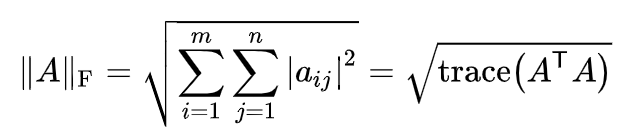
\includegraphics{image/textbook_solution_4.5.6.png}
  \caption{title}
  \end{figure}
\item
  \textbf{Review the relationship between training error and
  generalization error. In addition to weight decay, increased training,
  and the use of a model of suitable complexity, what other ways can you
  think of to deal with overfitting?}

  Add more training examples; Increase dropout; Decrease features, etc.
\item
  \textbf{In Bayesian statistics we use the product of prior and
  likelihood to arrive at a posterior via \(𝑝(𝑤|𝑥)∝𝑝(𝑥|𝑤)𝑝(𝑤)\) . How
  can you identify 𝑝(𝑤) with regularization?}
\end{enumerate}

    \paragraph{4.6.7. Exercises}\label{exercises}

\begin{enumerate}
\def\labelenumi{\arabic{enumi}.}
\tightlist
\item
  \textbf{Try out what happens if you change the dropout probabilities
  for layers 1 and 2. In particular, what happens if you switch the ones
  for both layers?}
\end{enumerate}

    \begin{Verbatim}[commandchars=\\\{\}]
{\color{incolor}In [{\color{incolor} }]:} \PY{c+c1}{\PYZsh{}\PYZsh{} TODO: Run on GPU}
        
        \PY{n}{num\PYZus{}epochs}\PY{p}{,} \PY{n}{lr}\PY{p}{,} \PY{n}{batch\PYZus{}size} \PY{o}{=} \PY{l+m+mi}{10}\PY{p}{,} \PY{l+m+mf}{0.5}\PY{p}{,} \PY{l+m+mi}{256}
        \PY{n}{loss} \PY{o}{=} \PY{n}{gloss}\PY{o}{.}\PY{n}{SoftmaxCrossEntropyLoss}\PY{p}{(}\PY{p}{)}
        \PY{n}{train\PYZus{}iter}\PY{p}{,} \PY{n}{test\PYZus{}iter} \PY{o}{=} \PY{n}{d2l}\PY{o}{.}\PY{n}{load\PYZus{}data\PYZus{}fashion\PYZus{}mnist}\PY{p}{(}\PY{n}{batch\PYZus{}size}\PY{p}{)}
        \PY{n}{drop\PYZus{}prob1}\PY{p}{,} \PY{n}{drop\PYZus{}prob2} \PY{o}{=} \PY{l+m+mf}{0.2}\PY{p}{,} \PY{l+m+mf}{0.5}
        
        \PY{c+c1}{\PYZsh{}\PYZsh{} network 1}
        \PY{n}{net467\PYZus{}1} \PY{o}{=} \PY{n}{nn}\PY{o}{.}\PY{n}{Sequential}\PY{p}{(}\PY{p}{)}
        \PY{n}{net467\PYZus{}1}\PY{o}{.}\PY{n}{add}\PY{p}{(}\PY{n}{nn}\PY{o}{.}\PY{n}{Dense}\PY{p}{(}\PY{l+m+mi}{256}\PY{p}{,} \PY{n}{activation}\PY{o}{=}\PY{l+s+s2}{\PYZdq{}}\PY{l+s+s2}{relu}\PY{l+s+s2}{\PYZdq{}}\PY{p}{)}\PY{p}{,}
                \PY{n}{nn}\PY{o}{.}\PY{n}{Dropout}\PY{p}{(}\PY{n}{drop\PYZus{}prob1}\PY{p}{)}\PY{p}{,}
                \PY{n}{nn}\PY{o}{.}\PY{n}{Dense}\PY{p}{(}\PY{l+m+mi}{256}\PY{p}{,} \PY{n}{activation}\PY{o}{=}\PY{l+s+s2}{\PYZdq{}}\PY{l+s+s2}{relu}\PY{l+s+s2}{\PYZdq{}}\PY{p}{)}\PY{p}{,}
                \PY{n}{nn}\PY{o}{.}\PY{n}{Dropout}\PY{p}{(}\PY{n}{drop\PYZus{}prob2}\PY{p}{)}\PY{p}{,}
                \PY{n}{nn}\PY{o}{.}\PY{n}{Dense}\PY{p}{(}\PY{l+m+mi}{10}\PY{p}{)}\PY{p}{)}
        \PY{n}{net467\PYZus{}1}\PY{o}{.}\PY{n}{initialize}\PY{p}{(}\PY{n}{init}\PY{o}{.}\PY{n}{Normal}\PY{p}{(}\PY{n}{sigma}\PY{o}{=}\PY{l+m+mf}{0.01}\PY{p}{)}\PY{p}{)}
        \PY{n}{trainer} \PY{o}{=} \PY{n}{gluon}\PY{o}{.}\PY{n}{Trainer}\PY{p}{(}\PY{n}{net467\PYZus{}1}\PY{o}{.}\PY{n}{collect\PYZus{}params}\PY{p}{(}\PY{p}{)}\PY{p}{,} \PY{l+s+s1}{\PYZsq{}}\PY{l+s+s1}{sgd}\PY{l+s+s1}{\PYZsq{}}\PY{p}{,} \PY{p}{\PYZob{}}\PY{l+s+s1}{\PYZsq{}}\PY{l+s+s1}{learning\PYZus{}rate}\PY{l+s+s1}{\PYZsq{}}\PY{p}{:} \PY{n}{lr}\PY{p}{\PYZcb{}}\PY{p}{)}
        \PY{n}{d2l}\PY{o}{.}\PY{n}{train\PYZus{}ch3}\PY{p}{(}\PY{n}{net467\PYZus{}1}\PY{p}{,} \PY{n}{train\PYZus{}iter}\PY{p}{,} \PY{n}{test\PYZus{}iter}\PY{p}{,} \PY{n}{loss}\PY{p}{,} \PY{n}{num\PYZus{}epochs}\PY{p}{,} \PY{n}{batch\PYZus{}size}\PY{p}{,} \PY{k+kc}{None}\PY{p}{,}
                      \PY{k+kc}{None}\PY{p}{,} \PY{n}{trainer}\PY{p}{)}
\end{Verbatim}


    \begin{Verbatim}[commandchars=\\\{\}]
{\color{incolor}In [{\color{incolor} }]:} \PY{c+c1}{\PYZsh{}\PYZsh{} TODO: Run on GPU}
        
        \PY{c+c1}{\PYZsh{}\PYZsh{} network 2, switch dropout rate}
        \PY{n}{net467\PYZus{}2} \PY{o}{=} \PY{n}{nn}\PY{o}{.}\PY{n}{Sequential}\PY{p}{(}\PY{p}{)}
        \PY{n}{net467\PYZus{}2}\PY{o}{.}\PY{n}{add}\PY{p}{(}\PY{n}{nn}\PY{o}{.}\PY{n}{Dense}\PY{p}{(}\PY{l+m+mi}{256}\PY{p}{,} \PY{n}{activation}\PY{o}{=}\PY{l+s+s2}{\PYZdq{}}\PY{l+s+s2}{relu}\PY{l+s+s2}{\PYZdq{}}\PY{p}{)}\PY{p}{,}
                \PY{n}{nn}\PY{o}{.}\PY{n}{Dropout}\PY{p}{(}\PY{n}{drop\PYZus{}prob2}\PY{p}{)}\PY{p}{,}
                \PY{n}{nn}\PY{o}{.}\PY{n}{Dense}\PY{p}{(}\PY{l+m+mi}{256}\PY{p}{,} \PY{n}{activation}\PY{o}{=}\PY{l+s+s2}{\PYZdq{}}\PY{l+s+s2}{relu}\PY{l+s+s2}{\PYZdq{}}\PY{p}{)}\PY{p}{,}
                \PY{n}{nn}\PY{o}{.}\PY{n}{Dropout}\PY{p}{(}\PY{n}{drop\PYZus{}prob1}\PY{p}{)}\PY{p}{,}
                \PY{n}{nn}\PY{o}{.}\PY{n}{Dense}\PY{p}{(}\PY{l+m+mi}{10}\PY{p}{)}\PY{p}{)}
        \PY{n}{net467\PYZus{}2}\PY{o}{.}\PY{n}{initialize}\PY{p}{(}\PY{n}{init}\PY{o}{.}\PY{n}{Normal}\PY{p}{(}\PY{n}{sigma}\PY{o}{=}\PY{l+m+mf}{0.01}\PY{p}{)}\PY{p}{)}
        \PY{n}{trainer} \PY{o}{=} \PY{n}{gluon}\PY{o}{.}\PY{n}{Trainer}\PY{p}{(}\PY{n}{net467\PYZus{}2}\PY{o}{.}\PY{n}{collect\PYZus{}params}\PY{p}{(}\PY{p}{)}\PY{p}{,} \PY{l+s+s1}{\PYZsq{}}\PY{l+s+s1}{sgd}\PY{l+s+s1}{\PYZsq{}}\PY{p}{,} \PY{p}{\PYZob{}}\PY{l+s+s1}{\PYZsq{}}\PY{l+s+s1}{learning\PYZus{}rate}\PY{l+s+s1}{\PYZsq{}}\PY{p}{:} \PY{n}{lr}\PY{p}{\PYZcb{}}\PY{p}{)}
        \PY{n}{d2l}\PY{o}{.}\PY{n}{train\PYZus{}ch3}\PY{p}{(}\PY{n}{net467\PYZus{}2}\PY{p}{,} \PY{n}{train\PYZus{}iter}\PY{p}{,} \PY{n}{test\PYZus{}iter}\PY{p}{,} \PY{n}{loss}\PY{p}{,} \PY{n}{num\PYZus{}epochs}\PY{p}{,} \PY{n}{batch\PYZus{}size}\PY{p}{,} \PY{k+kc}{None}\PY{p}{,}
                      \PY{k+kc}{None}\PY{p}{,} \PY{n}{trainer}\PY{p}{)}
\end{Verbatim}


    \begin{enumerate}
\def\labelenumi{\arabic{enumi}.}
\setcounter{enumi}{1}
\tightlist
\item
  \textbf{Increase the number of epochs and compare the results obtained
  when using dropout with those when not using it.}
\end{enumerate}

    \begin{Verbatim}[commandchars=\\\{\}]
{\color{incolor}In [{\color{incolor} }]:} \PY{c+c1}{\PYZsh{}\PYZsh{} TODO: Run on GPU}
        
        \PY{c+c1}{\PYZsh{}\PYZsh{} network 3}
        \PY{n}{num\PYZus{}epochs} \PY{o}{=} \PY{l+m+mi}{50}
        \PY{n}{net467\PYZus{}3} \PY{o}{=} \PY{n}{nn}\PY{o}{.}\PY{n}{Sequential}\PY{p}{(}\PY{p}{)}
        \PY{n}{net467\PYZus{}3}\PY{o}{.}\PY{n}{add}\PY{p}{(}\PY{n}{nn}\PY{o}{.}\PY{n}{Dense}\PY{p}{(}\PY{l+m+mi}{256}\PY{p}{,} \PY{n}{activation}\PY{o}{=}\PY{l+s+s2}{\PYZdq{}}\PY{l+s+s2}{relu}\PY{l+s+s2}{\PYZdq{}}\PY{p}{)}\PY{p}{,}
                \PY{n}{nn}\PY{o}{.}\PY{n}{Dropout}\PY{p}{(}\PY{n}{drop\PYZus{}prob2}\PY{p}{)}\PY{p}{,}
                \PY{n}{nn}\PY{o}{.}\PY{n}{Dense}\PY{p}{(}\PY{l+m+mi}{256}\PY{p}{,} \PY{n}{activation}\PY{o}{=}\PY{l+s+s2}{\PYZdq{}}\PY{l+s+s2}{relu}\PY{l+s+s2}{\PYZdq{}}\PY{p}{)}\PY{p}{,}
                \PY{n}{nn}\PY{o}{.}\PY{n}{Dropout}\PY{p}{(}\PY{n}{drop\PYZus{}prob1}\PY{p}{)}\PY{p}{,}
                \PY{n}{nn}\PY{o}{.}\PY{n}{Dense}\PY{p}{(}\PY{l+m+mi}{10}\PY{p}{)}\PY{p}{)}
        \PY{n}{net467\PYZus{}3}\PY{o}{.}\PY{n}{initialize}\PY{p}{(}\PY{n}{init}\PY{o}{.}\PY{n}{Normal}\PY{p}{(}\PY{n}{sigma}\PY{o}{=}\PY{l+m+mf}{0.01}\PY{p}{)}\PY{p}{)}
        \PY{n}{trainer} \PY{o}{=} \PY{n}{gluon}\PY{o}{.}\PY{n}{Trainer}\PY{p}{(}\PY{n}{net467\PYZus{}3}\PY{o}{.}\PY{n}{collect\PYZus{}params}\PY{p}{(}\PY{p}{)}\PY{p}{,} \PY{l+s+s1}{\PYZsq{}}\PY{l+s+s1}{sgd}\PY{l+s+s1}{\PYZsq{}}\PY{p}{,} \PY{p}{\PYZob{}}\PY{l+s+s1}{\PYZsq{}}\PY{l+s+s1}{learning\PYZus{}rate}\PY{l+s+s1}{\PYZsq{}}\PY{p}{:} \PY{n}{lr}\PY{p}{\PYZcb{}}\PY{p}{)}
        \PY{n}{d2l}\PY{o}{.}\PY{n}{train\PYZus{}ch3}\PY{p}{(}\PY{n}{net467\PYZus{}3}\PY{p}{,} \PY{n}{train\PYZus{}iter}\PY{p}{,} \PY{n}{test\PYZus{}iter}\PY{p}{,} \PY{n}{loss}\PY{p}{,} \PY{n}{num\PYZus{}epochs}\PY{p}{,} \PY{n}{batch\PYZus{}size}\PY{p}{,} \PY{k+kc}{None}\PY{p}{,}
                      \PY{k+kc}{None}\PY{p}{,} \PY{n}{trainer}\PY{p}{)}
\end{Verbatim}


    \begin{enumerate}
\def\labelenumi{\arabic{enumi}.}
\setcounter{enumi}{2}
\item
  \textbf{Compute the variance of the the activation random variables
  after applying dropout.}

  Dropout replaces an activation ℎ with a random variable ℎ′ with
  expected value ℎ and with variance given by the dropout probability 𝑝
  .

  \[\begin{split}\begin{aligned}
      h' =
      \begin{cases}
          0 & \text{ with probability } p \\
          \frac{h}{1-p} & \text{ otherwise}
      \end{cases}
      \end{aligned}\end{split}\]
\end{enumerate}

    \begin{enumerate}
\def\labelenumi{\arabic{enumi}.}
\setcounter{enumi}{3}
\item
  \textbf{Why should you typically not using dropout?}

  Dropout can help with regularization, but at a risk of lossing
  improtant information. Especially applying Dropout in the first layer
  will lead to significant inforamtion loss.
\item
  \textbf{If changes are made to the model to make it more complex, such
  as adding hidden layer units, will the effect of using dropout to cope
  with overfitting be more obvious?}
\end{enumerate}

??????

For an overfitted model, adding a hidden layer with dropout may not
help. Especially in the situation that the effective neurons in this
layer is larger than the number of neurons in the later layers, since
this is equal to adding an extra hidden layer.

\begin{enumerate}
\def\labelenumi{\arabic{enumi}.}
\setcounter{enumi}{5}
\tightlist
\item
  \textbf{Using the model in this section as an example, compare the
  effects of using dropout and weight decay. What if dropout and weight
  decay are used at the same time?}
\end{enumerate}

    \begin{Verbatim}[commandchars=\\\{\}]
{\color{incolor}In [{\color{incolor} }]:} \PY{c+c1}{\PYZsh{}\PYZsh{} TODO: Run on GPU}
        
        \PY{c+c1}{\PYZsh{}\PYZsh{} random simulate dataset}
        \PY{n}{n\PYZus{}train}\PY{p}{,} \PY{n}{n\PYZus{}test}\PY{p}{,} \PY{n}{num\PYZus{}inputs} \PY{o}{=} \PY{l+m+mi}{20}\PY{p}{,} \PY{l+m+mi}{100}\PY{p}{,} \PY{l+m+mi}{200}
        \PY{n}{true\PYZus{}w}\PY{p}{,} \PY{n}{true\PYZus{}b} \PY{o}{=} \PY{n}{nd}\PY{o}{.}\PY{n}{ones}\PY{p}{(}\PY{p}{(}\PY{n}{num\PYZus{}inputs}\PY{p}{,} \PY{l+m+mi}{1}\PY{p}{)}\PY{p}{)} \PY{o}{*} \PY{l+m+mf}{0.01}\PY{p}{,} \PY{l+m+mf}{0.05}
        
        \PY{n}{features} \PY{o}{=} \PY{n}{nd}\PY{o}{.}\PY{n}{random}\PY{o}{.}\PY{n}{normal}\PY{p}{(}\PY{n}{shape}\PY{o}{=}\PY{p}{(}\PY{n}{n\PYZus{}train} \PY{o}{+} \PY{n}{n\PYZus{}test}\PY{p}{,} \PY{n}{num\PYZus{}inputs}\PY{p}{)}\PY{p}{)}
        \PY{n}{labels} \PY{o}{=} \PY{n}{nd}\PY{o}{.}\PY{n}{dot}\PY{p}{(}\PY{n}{features}\PY{p}{,} \PY{n}{true\PYZus{}w}\PY{p}{)} \PY{o}{+} \PY{n}{true\PYZus{}b}
        \PY{n}{labels} \PY{o}{+}\PY{o}{=} \PY{n}{nd}\PY{o}{.}\PY{n}{random}\PY{o}{.}\PY{n}{normal}\PY{p}{(}\PY{n}{scale}\PY{o}{=}\PY{l+m+mf}{0.01}\PY{p}{,} \PY{n}{shape}\PY{o}{=}\PY{n}{labels}\PY{o}{.}\PY{n}{shape}\PY{p}{)}
        \PY{n}{train\PYZus{}features}\PY{p}{,} \PY{n}{test\PYZus{}features} \PY{o}{=} \PY{n}{features}\PY{p}{[}\PY{p}{:}\PY{n}{n\PYZus{}train}\PY{p}{,} \PY{p}{:}\PY{p}{]}\PY{p}{,} \PY{n}{features}\PY{p}{[}\PY{n}{n\PYZus{}train}\PY{p}{:}\PY{p}{,} \PY{p}{:}\PY{p}{]}
        \PY{n}{train\PYZus{}labels}\PY{p}{,} \PY{n}{test\PYZus{}labels} \PY{o}{=} \PY{n}{labels}\PY{p}{[}\PY{p}{:}\PY{n}{n\PYZus{}train}\PY{p}{]}\PY{p}{,} \PY{n}{labels}\PY{p}{[}\PY{n}{n\PYZus{}train}\PY{p}{:}\PY{p}{]}
        \PY{n}{train\PYZus{}iter} \PY{o}{=} \PY{n}{gdata}\PY{o}{.}\PY{n}{DataLoader}\PY{p}{(}\PY{n}{gdata}\PY{o}{.}\PY{n}{ArrayDataset}\PY{p}{(}\PY{n}{train\PYZus{}features}\PY{p}{,} \PY{n}{train\PYZus{}labels}\PY{p}{)}\PY{p}{,} \PY{n}{batch\PYZus{}size}\PY{p}{,} \PY{n}{shuffle}\PY{o}{=}\PY{k+kc}{True}\PY{p}{)}
        
        
        
        \PY{k}{def} \PY{n+nf}{fit\PYZus{}and\PYZus{}plot\PYZus{}gluon\PYZus{}467\PYZus{}6}\PY{p}{(}\PY{n}{dropout}\PY{p}{,} \PY{n}{wd}\PY{p}{,} \PY{n}{num\PYZus{}epochs}\PY{o}{=}\PY{l+m+mi}{50}\PY{p}{,} \PY{n}{lr}\PY{o}{=}\PY{l+m+mf}{0.01}\PY{p}{,} \PY{n}{batch\PYZus{}size}\PY{o}{=}\PY{l+m+mi}{256}\PY{p}{)}\PY{p}{:}
            \PY{n}{net} \PY{o}{=} \PY{n}{nn}\PY{o}{.}\PY{n}{Sequential}\PY{p}{(}\PY{p}{)}
            \PY{n}{net}\PY{o}{.}\PY{n}{add}\PY{p}{(}\PY{n}{nn}\PY{o}{.}\PY{n}{Dense}\PY{p}{(}\PY{l+m+mi}{256}\PY{p}{)}\PY{p}{,}
                    \PY{n}{nn}\PY{o}{.}\PY{n}{Dropout}\PY{p}{(}\PY{n}{drop\PYZus{}prob}\PY{p}{)}\PY{p}{,}
                    \PY{n}{nn}\PY{o}{.}\PY{n}{Dense}\PY{p}{(}\PY{l+m+mi}{10}\PY{p}{)}\PY{p}{)}
            \PY{n}{net}\PY{o}{.}\PY{n}{initialize}\PY{p}{(}\PY{n}{init}\PY{o}{.}\PY{n}{Normal}\PY{p}{(}\PY{n}{sigma}\PY{o}{=}\PY{l+m+mf}{0.01}\PY{p}{)}\PY{p}{)}
            \PY{n}{loss} \PY{o}{=} \PY{n}{gloss}\PY{o}{.}\PY{n}{L2Loss}\PY{p}{(}\PY{p}{)}
        
            \PY{n}{trainer\PYZus{}w} \PY{o}{=} \PY{n}{gluon}\PY{o}{.}\PY{n}{Trainer}\PY{p}{(}\PY{n}{net}\PY{o}{.}\PY{n}{collect\PYZus{}params}\PY{p}{(}\PY{l+s+s1}{\PYZsq{}}\PY{l+s+s1}{.*weight}\PY{l+s+s1}{\PYZsq{}}\PY{p}{)}\PY{p}{,} \PY{l+s+s1}{\PYZsq{}}\PY{l+s+s1}{sgd}\PY{l+s+s1}{\PYZsq{}}\PY{p}{,}
                                      \PY{p}{\PYZob{}}\PY{l+s+s1}{\PYZsq{}}\PY{l+s+s1}{learning\PYZus{}rate}\PY{l+s+s1}{\PYZsq{}}\PY{p}{:} \PY{n}{lr}\PY{p}{,} \PY{l+s+s1}{\PYZsq{}}\PY{l+s+s1}{wd}\PY{l+s+s1}{\PYZsq{}}\PY{p}{:} \PY{n}{wd}\PY{p}{\PYZcb{}}\PY{p}{)}
            \PY{c+c1}{\PYZsh{} The bias parameter has not decayed. Bias names generally end with \PYZdq{}bias\PYZdq{}}
            \PY{n}{trainer\PYZus{}b} \PY{o}{=} \PY{n}{gluon}\PY{o}{.}\PY{n}{Trainer}\PY{p}{(}\PY{n}{net}\PY{o}{.}\PY{n}{collect\PYZus{}params}\PY{p}{(}\PY{l+s+s1}{\PYZsq{}}\PY{l+s+s1}{.*bias}\PY{l+s+s1}{\PYZsq{}}\PY{p}{)}\PY{p}{,} \PY{l+s+s1}{\PYZsq{}}\PY{l+s+s1}{sgd}\PY{l+s+s1}{\PYZsq{}}\PY{p}{,}
                                      \PY{p}{\PYZob{}}\PY{l+s+s1}{\PYZsq{}}\PY{l+s+s1}{learning\PYZus{}rate}\PY{l+s+s1}{\PYZsq{}}\PY{p}{:} \PY{n}{lr}\PY{p}{\PYZcb{}}\PY{p}{)}
            \PY{n}{train\PYZus{}ls}\PY{p}{,} \PY{n}{test\PYZus{}ls} \PY{o}{=} \PY{p}{[}\PY{p}{]}\PY{p}{,} \PY{p}{[}\PY{p}{]}
            \PY{k}{for} \PY{n}{\PYZus{}} \PY{o+ow}{in} \PY{n+nb}{range}\PY{p}{(}\PY{n}{num\PYZus{}epochs}\PY{p}{)}\PY{p}{:}
                \PY{k}{for} \PY{n}{X}\PY{p}{,} \PY{n}{y} \PY{o+ow}{in} \PY{n}{train\PYZus{}iter}\PY{p}{:}
                    \PY{k}{with} \PY{n}{autograd}\PY{o}{.}\PY{n}{record}\PY{p}{(}\PY{p}{)}\PY{p}{:}
                        \PY{n}{l} \PY{o}{=} \PY{n}{loss}\PY{p}{(}\PY{n}{net}\PY{p}{(}\PY{n}{X}\PY{p}{)}\PY{p}{,} \PY{n}{y}\PY{p}{)}
                    \PY{n}{l}\PY{o}{.}\PY{n}{backward}\PY{p}{(}\PY{p}{)}
                    \PY{c+c1}{\PYZsh{} Call the step function on each of the two Trainer instances to}
                    \PY{c+c1}{\PYZsh{} update the weight and bias separately}
                    \PY{n}{trainer\PYZus{}w}\PY{o}{.}\PY{n}{step}\PY{p}{(}\PY{n}{batch\PYZus{}size}\PY{p}{)}
                    \PY{n}{trainer\PYZus{}b}\PY{o}{.}\PY{n}{step}\PY{p}{(}\PY{n}{batch\PYZus{}size}\PY{p}{)}
                \PY{n}{train\PYZus{}ls}\PY{o}{.}\PY{n}{append}\PY{p}{(}\PY{n}{loss}\PY{p}{(}\PY{n}{net}\PY{p}{(}\PY{n}{train\PYZus{}features}\PY{p}{)}\PY{p}{,}
                                     \PY{n}{train\PYZus{}labels}\PY{p}{)}\PY{o}{.}\PY{n}{mean}\PY{p}{(}\PY{p}{)}\PY{o}{.}\PY{n}{asscalar}\PY{p}{(}\PY{p}{)}\PY{p}{)}
                \PY{n}{test\PYZus{}ls}\PY{o}{.}\PY{n}{append}\PY{p}{(}\PY{n}{loss}\PY{p}{(}\PY{n}{net}\PY{p}{(}\PY{n}{test\PYZus{}features}\PY{p}{)}\PY{p}{,}
                                    \PY{n}{test\PYZus{}labels}\PY{p}{)}\PY{o}{.}\PY{n}{mean}\PY{p}{(}\PY{p}{)}\PY{o}{.}\PY{n}{asscalar}\PY{p}{(}\PY{p}{)}\PY{p}{)}
            \PY{n}{d2l}\PY{o}{.}\PY{n}{semilogy}\PY{p}{(}\PY{n+nb}{range}\PY{p}{(}\PY{l+m+mi}{1}\PY{p}{,} \PY{n}{num\PYZus{}epochs} \PY{o}{+} \PY{l+m+mi}{1}\PY{p}{)}\PY{p}{,} \PY{n}{train\PYZus{}ls}\PY{p}{,} \PY{l+s+s1}{\PYZsq{}}\PY{l+s+s1}{epochs}\PY{l+s+s1}{\PYZsq{}}\PY{p}{,} \PY{l+s+s1}{\PYZsq{}}\PY{l+s+s1}{loss}\PY{l+s+s1}{\PYZsq{}}\PY{p}{,}
                         \PY{n+nb}{range}\PY{p}{(}\PY{l+m+mi}{1}\PY{p}{,} \PY{n}{num\PYZus{}epochs} \PY{o}{+} \PY{l+m+mi}{1}\PY{p}{)}\PY{p}{,} \PY{n}{test\PYZus{}ls}\PY{p}{,} \PY{p}{[}\PY{l+s+s1}{\PYZsq{}}\PY{l+s+s1}{train}\PY{l+s+s1}{\PYZsq{}}\PY{p}{,} \PY{l+s+s1}{\PYZsq{}}\PY{l+s+s1}{test}\PY{l+s+s1}{\PYZsq{}}\PY{p}{]}\PY{p}{)}
        \PY{c+c1}{\PYZsh{}     print(\PYZsq{}L2 norm of w:\PYZsq{}, net[0].weight.data().norm().asscalar())}
        
        \PY{n}{fit\PYZus{}and\PYZus{}plot\PYZus{}gluon\PYZus{}467\PYZus{}6}\PY{p}{(}\PY{n}{dropout}\PY{o}{=}\PY{l+m+mf}{0.5}\PY{p}{,} \PY{n}{wd}\PY{o}{=}\PY{l+m+mi}{0}\PY{p}{)} 
        \PY{n}{fit\PYZus{}and\PYZus{}plot\PYZus{}gluon\PYZus{}467\PYZus{}6}\PY{p}{(}\PY{n}{dropout}\PY{o}{=}\PY{l+m+mf}{0.5}\PY{p}{,} \PY{n}{wd}\PY{o}{=}\PY{l+m+mi}{3}\PY{p}{)}
        \PY{n}{fit\PYZus{}and\PYZus{}plot\PYZus{}gluon\PYZus{}467\PYZus{}6}\PY{p}{(}\PY{n}{dropout}\PY{o}{=}\PY{l+m+mi}{0}\PY{p}{,} \PY{n}{wd}\PY{o}{=}\PY{l+m+mi}{3}\PY{p}{)} 
\end{Verbatim}


    \begin{enumerate}
\def\labelenumi{\arabic{enumi}.}
\setcounter{enumi}{6}
\item
  \textbf{What happens if we apply dropout to the individual weights of
  the weight matrix rather than the activations?}

  The regularization effect will be the same. If we turn partial of the
  weights to be zero, these neurons won't learn any signal from the
  inputs, which will have the similar functionality as dropout on
  activation.
\item
  \textbf{Replace the dropout activation with a random variable that
  takes on values of \([0,\gamma/2,\gamma]\) . Can you design something
  that works better than the binary dropout function? Why might you want
  to use it? Why not?}

  Define the following dropout activation function:

  \[\begin{split}\begin{aligned}
  h' =
  \begin{cases}
      0 & \text{ with probability } p_1 \\
      \gamma/2 * h & \text{ with probability } (1 - p_1)  p_2 \\
      \gamma * h & \text{ with probability } (1 - p_1)(1 - p_2)
  \end{cases}
  \end{aligned}\end{split}\]

  The has the expectation remained unchanged, we need to have
  \[ 0 + (\gamma/2) h (1 - p_1)  p_2 +  \gamma  h  (1 - p_1)(1 - p_2)  = h\]
  Thus, \[\gamma = \frac{2}{(2-p_2)(1-p_1)}\]

  For example, if we let \(p_1=0.2, p_2=0.75\), then \(\gamma = 2\) by
  the above formula,

  \[\begin{split}\begin{aligned}
  h' =
  \begin{cases}
      0 & \text{ with probability } 0.2 \\
      h & \text{ with probability } 0.6 \\
      2 h & \text{ with probability } 0.2
  \end{cases}
  \end{aligned}\end{split}\]
\end{enumerate}

    \paragraph{4.7.6. Exercises}\label{exercises}

\begin{enumerate}
\def\labelenumi{\arabic{enumi}.}
\item
  \textbf{Assume that the inputs X are matrices. What is the
  dimensionality of the gradients?}

  Notice the dimensionality of each layer's graditents is equal the
  dimensionality of each layer's weighs. i.e.
  \[ dim(\frac{\partial J}{\partial \mathbf{W}^{(1)}}) = dim(\mathbf{W}^{(1)})\]

  If the inputs \(X \in \mathbb{R}^{d \times c}\) are matrices at each
  row, the weight matrix \(\mathbf{W}^{(1)}\) would have a dimension
  equal to \({h \times (d \times c)}\), where h is the hidden layer
  dimension.
\item
  \textbf{Add a bias to the hidden layer of the model described in this
  chapter.}

  \begin{enumerate}
  \def\labelenumii{\alph{enumii}.}
  \item
    \textbf{Draw the corresponding compute graph.}
  \item
    \textbf{Derive the forward and backward propagation equations.}
  \item
    Given a hidden layer with a bias:
    \[\mathbf{z}= \mathbf{W}^{(1)} \mathbf{x} + \mathbf{b}^{(1)}\\
      \mathbf{h}= \phi (\mathbf{z}) \\
      \mathbf{o}= \mathbf{W}^{(2)} \mathbf{h} + \mathbf{b}^{(2)}\\
      L = l(\mathbf{o}, y) \\
      s = \frac{\lambda}{2} \left(\|\mathbf{W}^{(1)}\|_F^2 + \|\mathbf{W}^{(2)}\|_F^2\right) \\
      J = L + s\]
  \end{enumerate}

  hence the backward propagation will be
  \[ \frac{\partial J}{\partial \mathbf{W}^{(2)}}
      = \text{prod}\left(\frac{\partial J}{\partial \mathbf{o}}, \frac{\partial \mathbf{o}}{\partial \mathbf{W}^{(2)}}\right) + \text{prod}\left(\frac{\partial J}{\partial s}, \frac{\partial s}{\partial \mathbf{W}^{(2)}}\right)
      = \frac{\partial J}{\partial \mathbf{o}} \mathbf{h}^\top + \lambda \mathbf{W}^{(2)}\]

  \[ \frac{\partial J}{\partial \mathbf{b}^{(2)}}
      = \text{prod}\left(\frac{\partial J}{\partial \mathbf{o}}, \frac{\partial \mathbf{o}}{\partial \mathbf{b}^{(2)}}\right)  + \text{prod}\left(\frac{\partial J}{\partial s}, \frac{\partial s}{\partial \mathbf{b}^{(2)}}\right)
      = \frac{\partial J}{\partial \mathbf{o}} \times 1 + 0
      = \frac{\partial J}{\partial \mathbf{o}}\]
  \[ \frac{\partial J}{\partial \mathbf{W}^{(1)}}
      = \frac{\partial J}{\partial \mathbf{o}} \frac{\partial \mathbf{o}}{\partial \mathbf{h}} \frac{\partial \mathbf{h}}{\partial \mathbf{z}} \frac{\partial \mathbf{z}}{\partial \mathbf{W}^{(1)}} + \text{prod}\left(\frac{\partial J}{\partial s}, \frac{\partial s}{\partial \mathbf{W}^{(1)}}\right)
      = \frac{\partial J}{\partial \mathbf{o}} {\mathbf{W}^{(2)}}^\top \odot \phi'\left(\mathbf{z}\right) {\mathbf{x}}^\top + \lambda \mathbf{W}^{(1)}\]

  \[ \frac{\partial J}{\partial \mathbf{b}^{(1)}}
      = \frac{\partial J}{\partial \mathbf{o}} \frac{\partial \mathbf{o}}{\partial \mathbf{h}} \frac{\partial \mathbf{h}}{\partial \mathbf{z}} \frac{\partial \mathbf{z}}{\partial \mathbf{b}^{(1)}} + \text{prod}\left(\frac{\partial J}{\partial s}, \frac{\partial s}{\partial \mathbf{b}^{(1)}}\right)
      = \frac{\partial J}{\partial \mathbf{o}} {\mathbf{W}^{(2)}}^\top \odot \phi'\left(\mathbf{z}\right)\]
\end{enumerate}

    \begin{enumerate}
\def\labelenumi{\arabic{enumi}.}
\setcounter{enumi}{2}
\item
  \textbf{Compute the memory footprint for training and inference in
  model described in the current chapter.}

  Training: need memory for
  \[ \frac{\partial J}{\partial \mathbf{o}}, {\mathbf{W}^{(2)}}, {\mathbf{W}^{(1)}}, \phi'\left(\mathbf{z}\right), {\mathbf{x}},\]
  Inference: only need memory for
  \[\mathbf{W}^{(1)}, \mathbf{W}^{(2)}, \mathbf{b}^{(1)}, \mathbf{b}^{(2)}\]
\item
  \textbf{Assume that you want to compute second derivatives. What
  happens to the compute graph? Is this a good idea?}
\item
  \textbf{Assume that the compute graph is too large for your GPU.}

  a.\textbf{Can you partition it over more than one GPU?}

\begin{verbatim}
By default, MXNet uses data parallelism to partition the workload over multiple devices. Assume there are n devices. Then each one will receive a copy of the complete model and train it on 1/n of the data. The results such as gradients and updated model are communicated across these devices.
\end{verbatim}

  b.\textbf{What are the advantages and disadvantages over training on a
  smaller minibatch?}

  Advantages: 1. More robust convergence, avoiding local minima (as its
  model update frequency is higher than batch gradient descent.) 2.
  Computationally efficient process than stochastic gradient descent. 3.
  Memory efficient than batch gradient descent.

  Disadvantages: 1. Tune minibatch hyperparameter
\end{enumerate}

    \paragraph{4.8.4. Exercises}\label{exercises}

\begin{enumerate}
\def\labelenumi{\arabic{enumi}.}
\item
  \textbf{Can you design other cases of symmetry breaking besides the
  permutation symmetry?}
\item
  \textbf{Can we initialize all weight parameters in linear regression
  or in softmax regression to the same value?}
\item
  \textbf{Look up analytic bounds on the eigenvalues of the product of
  two matrices. What does this tell you about ensuring that gradients
  are well conditioned?}
\item
  \textbf{If we know that some terms diverge, can we fix this after the
  fact? Look at the paper on LARS by You, Gitman and Ginsburg, 2017 for
  inspiration.}
\end{enumerate}

    \paragraph{4.9.5. Exercises}\label{exercises}

\begin{enumerate}
\def\labelenumi{\arabic{enumi}.}
\item
  \textbf{What could happen when we change the behavior of a search
  engine? What might the users do? What about the advertisers?}
\item
  \textbf{Implement a covariate shift detector. Hint - build a
  classifier.}
\item
  \textbf{Implement a covariate shift corrector.}
\item
  \textbf{What could go wrong if training and test set are very
  different? What would happen to the sample weights?}
\end{enumerate}


    % Add a bibliography block to the postdoc
    
    
    
    \end{document}
